% The code is also hosted at GitHub[1].
%
% [1] https://github.com/adityasz/cs217-lec-1

\documentclass[twoside]{article}
    \setlength{\oddsidemargin} {0.25 in}
    \setlength{\evensidemargin}{-0.25 in}
    \setlength{\topmargin}     {-0.6 in}
    \setlength{\textwidth}     {6.5 in}
    \setlength{\textheight}    {8.5 in}
    \setlength{\headsep}       {0.75 in}
    \setlength{\parindent}     {0 in}
    \setlength{\parskip}       {0.1 in}

\usepackage{amsmath}
\usepackage{amsfonts}
\usepackage{graphicx}
\usepackage{amssymb}
\usepackage{mathrsfs}   % provides \mathscr
\usepackage{physics}    % provides \norm
\usepackage{tikz}
    \usetikzlibrary{arrows.meta}
\usepackage{pgfplots}
    \pgfplotsset{compat=1.18}

%
% The following commands set up the lecnum (lecture number)
% counter and make various numbering schemes work relative
% to the lecture number.
%
\newcounter{lecnum}
\renewcommand{\thepage}    {\thelecnum-\arabic{page}}
\renewcommand{\thesection} {\thelecnum.\arabic{section}}
\renewcommand{\theequation}{\thelecnum.\arabic{equation}}
\renewcommand{\thefigure}  {\thelecnum.\arabic{figure}}
\renewcommand{\thetable}   {\thelecnum.\arabic{table}}

%
% The following macro is used to generate the header.
%
\newcommand{\lecture}[4]{
    \pagestyle{myheadings}
    \thispagestyle{plain}
    \newpage
    \setcounter{lecnum}{#1}
    \setcounter{page}{1}
    \noindent
    \begin{center}
        \framebox{
            \vbox{
                \vspace{2mm}
                \hbox to 6.28in {\textbf{CS 217: Artificial Intelligence and
                                  Machine Learning \hfill Jan 10, 2024}}
                \vspace{4mm}
                \hbox to 6.28in {{\Large \hfill Lecture #1: #2  \hfill}}
                \vspace{2mm}
                \hbox to 6.28in {\textit{Lecturer: #3 \hfill Scribes: #4}}
                \vspace{2mm}
            }
        }
    \end{center}
    \markboth{Lecture #1: #2}{Lecture #1: #2}

    \textbf{Disclaimer:} \textit{These notes aggregate content from several
    texts and have not been subjected to the usual scrutiny deserved by
    formal publications. If you find errors, please bring to the notice of
    the Instructor.}

    \vspace*{1mm}
}

%
% Convention for citations is authors' initials followed by the year.
% For example, to cite a paper by Leighton and Maggs you would type
% \cite{LM89}, and to cite a paper by Strassen you would type \cite{S69}.
% (To avoid bibliography problems, for now we redefine the \cite command.)
% Also commands that create a suitable format for the reference list.
%
\renewcommand{\cite}[1]{[#1]}
    \def\beginrefs{\begin{list}%
            {[\arabic{equation}]}{\usecounter{equation}
             \setlength{\leftmargin}{2.0truecm}\setlength{\labelsep}{0.4truecm}%
             \setlength{\labelwidth}{1.6truecm}}}
    \def\endrefs{\end{list}}
    \def\bibentry#1{\item[\hbox{[#1]}]}

% Use this command for a figure; it puts a figure in wherever you want it.
% usage: \fig{NUMBER}{JUST-THE-FILENAME}{CAPTION}
\newcommand{\fig}[3]{
    % \vspace{#2}
    \begin{center}
    \includegraphics{figures/#2}
    \newline
    Figure \thelecnum.#1:~#3
    \end{center}
}
	
% Use these for theorems, lemmas, proofs, etc.
\newtheorem{theorem}{Theorem}[lecnum]
\newtheorem{lemma}[theorem]{Lemma}
\newtheorem{proposition}[theorem]{Proposition}
\newtheorem{claim}[theorem]{Claim}
\newtheorem{corollary}[theorem]{Corollary}
\newtheorem{definition}[theorem]{Definition}
\newenvironment{proof}{{\textit{Proof.}}}{\hfill\rule{2mm}{2mm}}

\newcommand\R{\mathbb{R}}

\begin{document}

\lecture{1}{The Basics of Optimization}{Swaprava Nath}{Aditya Singh, Dion Reji,
Shreyas Katdare, Brian Mackwan}

In this lecture, we discuss what essentially optimization is, where we use
optimization, and look at a very basic optimization technique called linear
programming.

Broadly, optimization problems can be classified into two classes:

% TODO: Remove hardcoded values
\begin{table}[h]
    \centering
    \begin{tabular}{l | c | p{13 mm} | p{35 mm}}
        % \hline
        \textbf{Class}          & \textbf{Variable}
                                & \textbf{Solution space}
                                & \textbf{Solution complexity} \\
        \hline
        Continuous optimization & continuous
                                & infinite
                                & polynomial in the size of the problem \\
        \hline
        Discrete optimization   & discrete
                                & finite
                                & exponential in the size of the problem \\
        % \hline
    \end{tabular}
    \label{Classes of optimization problems.}
\end{table}

The knapsack problem is a classic discrete optimization problem, where we are
given a bunch of objects with specific weights and a knapsack (backpack, for
instance), which can carry at most some amount of weight. We want to fill our
knapsack up to the highest permissible weight. There is nothing like partial
association of an item with the knapsack: An item is either in the knapsack or
not. A polynomial solution to the most general knapsack problem is not known.
One way to solve it is to brute force all possible combinations and find the
optimal one, but this is not efficient.

In continuous optimization problems, even though the solution space is infinite,
it is not very difficult to find the optimal solution. We will be talking about
continuous optimization problems.

There is a significant trend in AI of formulating problems in terms of
optimization problems.

\section{What is optimization?}
There are two components of an optimization problem: The objective function
which we want to minimize (or maximize, which is just the negative of the
minimization problem), and the constraint set. Let $f(x)$ be the objective
function, and $\mathscr{C}$ be the constraint set.  Then, the optimization
problem is written as \[
    \min_{x \in \mathscr{C}} f(x).
\]

\textbf{Example.} Minimize $(x - 2)^2$ with the constraint that
$x \in [0, 1] \cup [4, 7].$

Here, the objective function is $f(x) = (x - 2)^2$ and the constraint set is
$\mathscr{C} = [0, 1] \cup [4, 7].$ This is a one-variable function, and we can
easily see from the plot in figure \ref{fig:ex1} that $x^* = 1$ is the optimal
value of $x$.

\begin{figure}[t]
    \centering
    \begin{tikzpicture}[scale=1, >=latex]
        \begin{axis} [
                axis x line = bottom,
                axis y line = none,
                xlabel = $x$,
                xmin   = -5,
                xmax   = 9,
                ymin   = 0,
                ymax   = 64,
                xtick  = {0, 1, 4, ..., 7},
                ytick  = {},
                width  = 60 mm,
                height = 40 mm,
                axis line style = {<->, >={Triangle[length=2mm, width=1.5mm]}}
            ]
            \addplot [line width = 1 pt]
                expression[
                    smooth,
                    samples = 2000,
                    domain  = -5:9
                ] {(x - 2) * (x - 2)};
        \end{axis}
    \end{tikzpicture}
    \caption{A plot of $f(x) = (x - 2)^2.$}
    \label{fig:ex1}
\end{figure}

\textbf{Example} (Geometry)\textbf{.} Suppose we have a map of a country with
cities represented by the points $\mathbf{y}_1, \ldots, \mathbf{y}_n$ in
two-dimensions. We want to set up a supply chain and deliver to all these
cities. We want to build a warehouse such that the sum of the distances from it
to all the cities is minimized (assuming we can transport the Euclidean way).

Let the warehouse be located at $\mathbf{x}.$ Then, the optimization problem is
\[
    \min_{\mathbf{x} \in \mathscr{C}}
        \sum_{i = 1}^{m} \|\mathbf{x} - \mathbf{y}_i\|_2,
\] where $\mathscr{C}$ is the set of all points in the country, and
$\| \mathbf{x} \|_2 = \sqrt{x_1^2 + x_2^2}$ represents the $L^2$ norm of
$\mathbf{x} = (x_1, x_2).$

% Insert figure

\textbf{Example} (Computer vision)\textbf{.} Image de-blurring is a common
problem in computer vision. We want to de-blur a blurred image according to some
policy.

We consider grayscale images of size $m \times n$, where each pixel has an
intensity value in $[0, 1]$: 0 meaning black, and 1 meaning white.  Let
$\mathbf{y} = [y_{i, j}]^{m \times n}$ be the blurred image that we are given.
Let $\mathbf{x} = [x_{i, j}]^{m \times n}$ be the original image and
$\mathbf{k}$ be the blurring filter which was applied to get $\mathbf{y}$.
Then, to get the original (de-blurred) image, we have to solve \[
    \min_{\mathbf{x} \in [0, 1]^{m \times n}}
    \left(
        \sum_{i = 0}^{m - 1} \sum_{j = 0}^{n - 1}
            |y_{i, j} - (\mathbf{k} * \mathbf{x})_{i, j}|
        + \lambda \sum_{i = 0}^{m - 1} \sum_{j = 0}^{n - 1}
            \underbrace{
                \left((x_{i, j} - x_{i, j + 1})^2
                      + (x_{i + 1, j} - x_{i, j})^2\right)
            }_{
                \text{to reduce sudden intensity changes}
            }
    \right).
\] $\lambda$ and $\mathbf{k}$ are the hyperparameters. $\lambda$ penalizes a
high difference in intensity of adjacent pixels.

\textbf{Example} (Machine learning)\textbf{.} Suppose we have inputs
$(x_i, y_i)$ for $i \in [n].$ We are trying to fit a curve through these points.
Suppose that we hypothesize the curve to be a polynomial
$h_{\boldsymbol{\theta}}(x) = w_0 + w_1x + w_2x^2$, where
$\boldsymbol\theta = (w_0, w_1, w_2)$ is a vector of the parameters. For each
point $x_i$, we want the hypothesized point $h_{\boldsymbol{\theta}}(x_i)$ to be
close to $y_i$. Let $\ell(x, y) = (x - y)^2$ be a (very simple) loss function.
Our objective is to minimize the sum of the loss over all the observed points.

The optimization problem is \[
    \min_{\boldsymbol{\theta} \in \R^3}
        \sum_{i = 1}^{n} \ell(h_{\boldsymbol{\theta}}(x_i), y_i).
\]
% Insert figure

\subsection{Linear Programming: An optimization type}
A linear program is a simple optimization type where the objective function and
constraints are given by linear relationships.

\textbf{Example} (Political Winning). Investing money to win the election

Consider a political scenario where a political party $P$ needs to invest money
to win elections. There are 3 different demographic classes, class 1, class 2,
and class 3, and four issues to be addressed: A, B, C, and D. There is a
specific pattern in which people from different classes respond to different
issues. Table \ref{tab:election_grid} contains the number of votes gained or
lost by the political party in each class per unit money spent on an issue, the
population of each class, and the majority required by the party to win in each
class.

\begin{table}[htbp]
    \centering
    \begin{tabular}{|c|c|c|c|}
        \hline
        \multicolumn{1}{|r|}{} & \multicolumn{3}{c|}{Classes} \\
        \hline
        Issues & Class$_1$ & Class$_2$ & Class$_3$  \\
        \hline
        A & $-2$ & 5 & 3 \\
        \hline
        B &  8   & 2 & $-5$ \\
        \hline
        C &  0   & 0 & 10 \\
        \hline
        D & 10   & 0 & 2 \\
        \hline
        Population & $100\,000$ & $200\,000$ & $50\,000$\\
        \hline
        Majority   &  $50\,000$ & $100\,000$ & $25\,000$\\
        \hline
    \end{tabular}
    \label{tab:election_grid}
    \caption{} % TODO: add some caption
\end{table}

The aim of the political party is to minimize the total amount of money it needs
to invest, yet get the required majority across each class. Let $x_1, x_2, x_3,
x_4$ be the amount of money the party invests in issues A, B, C, and D
respectively. Then, we have the following optimization problem: \[
    \min_{x_1, x_2, x_3, x_4} x_1 + x_2 + x_3 + x_4
\] subject to the constraints
% TODO: Align numbers without using phantom text.
\begin{align}
    -2x_1 + 8x_2 +  \phantom{1}0x_3 + 10x_4 &\geq \phantom{1}50\,000,  \label{eq:1} \\
    \phantom{-}5x_1 + 2x_2 +  \phantom{1}0x_3 +  \phantom{1}0x_4 &\geq 100\,000, \label{eq:2} \\
    \phantom{-}3x_1 + 5x_2 + 10x_3 +  \phantom{1}2x_4 &\geq \phantom{1}25\,000,  \label{eq:3}
\end{align}
and $x_1, x_2, x_3, x_4 \geq 0.$ Let us look at the optimal solution \[
    x_1^* = \frac{2\,050\,000}{111},\ x_2^* = \frac{425\,000}{111},\
    x_3^* = 0,\ x_4^* = \frac{625\,000}{111}.
\]

The optimal value of
$x_1 + x_2 + x_3 + x_4 = x_1^* + x_2^* + x_3^* + x_4^* = 3\,100\,000/111.$

After multiplying and adding the equations as
$(\ref{eq:1}) \cdot 25/222 + (\ref{eq:2}) \cdot 46/222 + (\ref{eq:3}) \cdot 14/222$,
we get \[
        x_1 + x_2 + \frac{140}{222}x_3 + x_4 \geq \frac{3\,100\,000}{111}.
\] Since
$x_1 + x_2 + x_3 + x_4 = x_1 + x_2 + 140 x_3/222 + x_4 \geq 3\,100\,000/111,$
this proves that our given solution is truly the optimal solution.

\subsection{Standard Form of Linear Program}
Let $\mathbf{x}$ be the vector containing the variables to optimize and $\mathbf{c}$
be the vector of constants: \[
    \mathbf{x} = \begin{bmatrix} x_1 \\ x_2 \\ \vdots \\ x_n \end{bmatrix},
    \quad
    \mathbf{c} = \begin{bmatrix} c_1 \\ c_2 \\ \vdots \\ c_n \end{bmatrix}.
\] Then, we can write the standard form of linear program as
$\max \mathbf{c}^\top \mathbf{x}$ subject to the constraints \[
    \mathbf{A}_{m \times n} \mathbf{x}_{n \times 1}
        \leq \mathbf{b}_{m \times 1}
        = \begin{bmatrix} b_1 \\ b_2 \\ \vdots \\ b_m \end{bmatrix},
\]
where $\mathbf{x} \geq \mathbf{0}.$ $\geq$ represents element-wise greater than or
equal to: \[
    \begin{bmatrix} x_1 \\ x_2 \\ \vdots \\ x_n \end{bmatrix}
        \geq \begin{bmatrix} 0 \\ 0 \\ \vdots \\ 0 \end{bmatrix}
    \iff \forall i,\ x_i \geq 0.
\]

The aforementioned problem is commonly referred to as the primal problem, and it
is accompanied by a corresponding dual problem.\\

\begin{minipage}[t]{0.45\textwidth}
  \centering
  \textbf{Primal Problem (P1)}
  \begin{align*}
    \text{maximize} \quad & \mathbf{c}^\top \mathbf{x} \\
    \text{subject to} \quad & \mathbf{Ax} \leq \mathbf{b} \\
    & \mathbf{x} \geq \mathbf{0}
  \end{align*}
\end{minipage}
\hfill
\begin{minipage}[t]{0.45\textwidth}
  \centering
  \textbf{Dual Problem (P2)}
  \begin{align*}
    \text{minimize} \quad & \mathbf{b}^\top \mathbf{y} \\
    \text{subject to} \quad & \mathbf{A}^\top \mathbf{y} \geq \mathbf{c} \\
    & \mathbf{y} \geq \mathbf{0}
  \end{align*}
\end{minipage}

\subsection{Weak Duality Principle}

\begin{theorem}[Weak Duality Principle]
    Let $\mathbf{x}$ and $\mathbf{y}$ represent feasible solutions, i.e., solutions
    that satisfy all the constraints, for the primal and dual problems,
    respectively. Then, \[
        \mathbf{b}^\top \mathbf{y} \ge \mathbf{c}^\top \mathbf{x}.
    \]
\end{theorem}
\begin{proof}
    \begin{align}
        \mathbf{Ax} &\leq \mathbf{b} \\
        \mathbf{x}^\top \mathbf{A}^\top &\leq \mathbf{b}^\top \\
        \intertext{
            As $\mathbf{y} \geq \mathbf{0}$, multiplying it on both sides will not
            change the inequality:
        }
        \mathbf{x}^\top \mathbf{A}^\top \mathbf{y}
                                        &\leq \mathbf{b}^\top \mathbf{y} \\
        \intertext{
            Since $\mathbf{A}^\top \mathbf{y} \geq \mathbf{c},$
        }
        \mathbf{b}^\top \mathbf{y} &\geq \mathbf{x}^\top \mathbf{c},
    \end{align}
    which can also be written as $\mathbf{b}^\top \mathbf{y} \geq
    \mathbf{c}^\top \mathbf{x}$.
    Thus, weak duality principle provides a relation between the
    solutions of primal and dual problems.
\end{proof}

\subsection{Strong Duality Theorem}
If a linear programming problem has an optimal solution, so does its dual. If
$\mathbf{x^*}$ and $\mathbf{y^*}$ are the optimal solutions of the primal and
dual problems respectively, then \[
    \mathbf{b}^\top \mathbf{y}^* = \mathbf{c}^\top \mathbf{x}^*.
\]

\end{document}
